\begin{frame}[allowframebreaks]{Rotation Prediction}
    \textbf{Rotation Prediction} is commonly used to learn useful image representations without requiring manual labels.
    \begin{itemize}
        \item \textbf{Task:} Rotate input images by a set of predefined angles (e.g., $0^\circ$, $90^\circ$, $180^\circ$, $270^\circ$).
        \item \textbf{Objective:} Train a neural network to predict the rotation angle applied to each image.
        \item \textbf{Implementation Steps:}
        \begin{itemize}
            \item Randomly select a rotation angle from the set.
            \item Apply the rotation to the input image.
            \item Feed the rotated image into the network.
            \item Use a classification head to predict the rotation angle.
            \item Compute the loss (e.g., cross-entropy) and update the model.
        \end{itemize}
    \end{itemize}

    \framebreak

    \begin{figure}
        \flushleft
        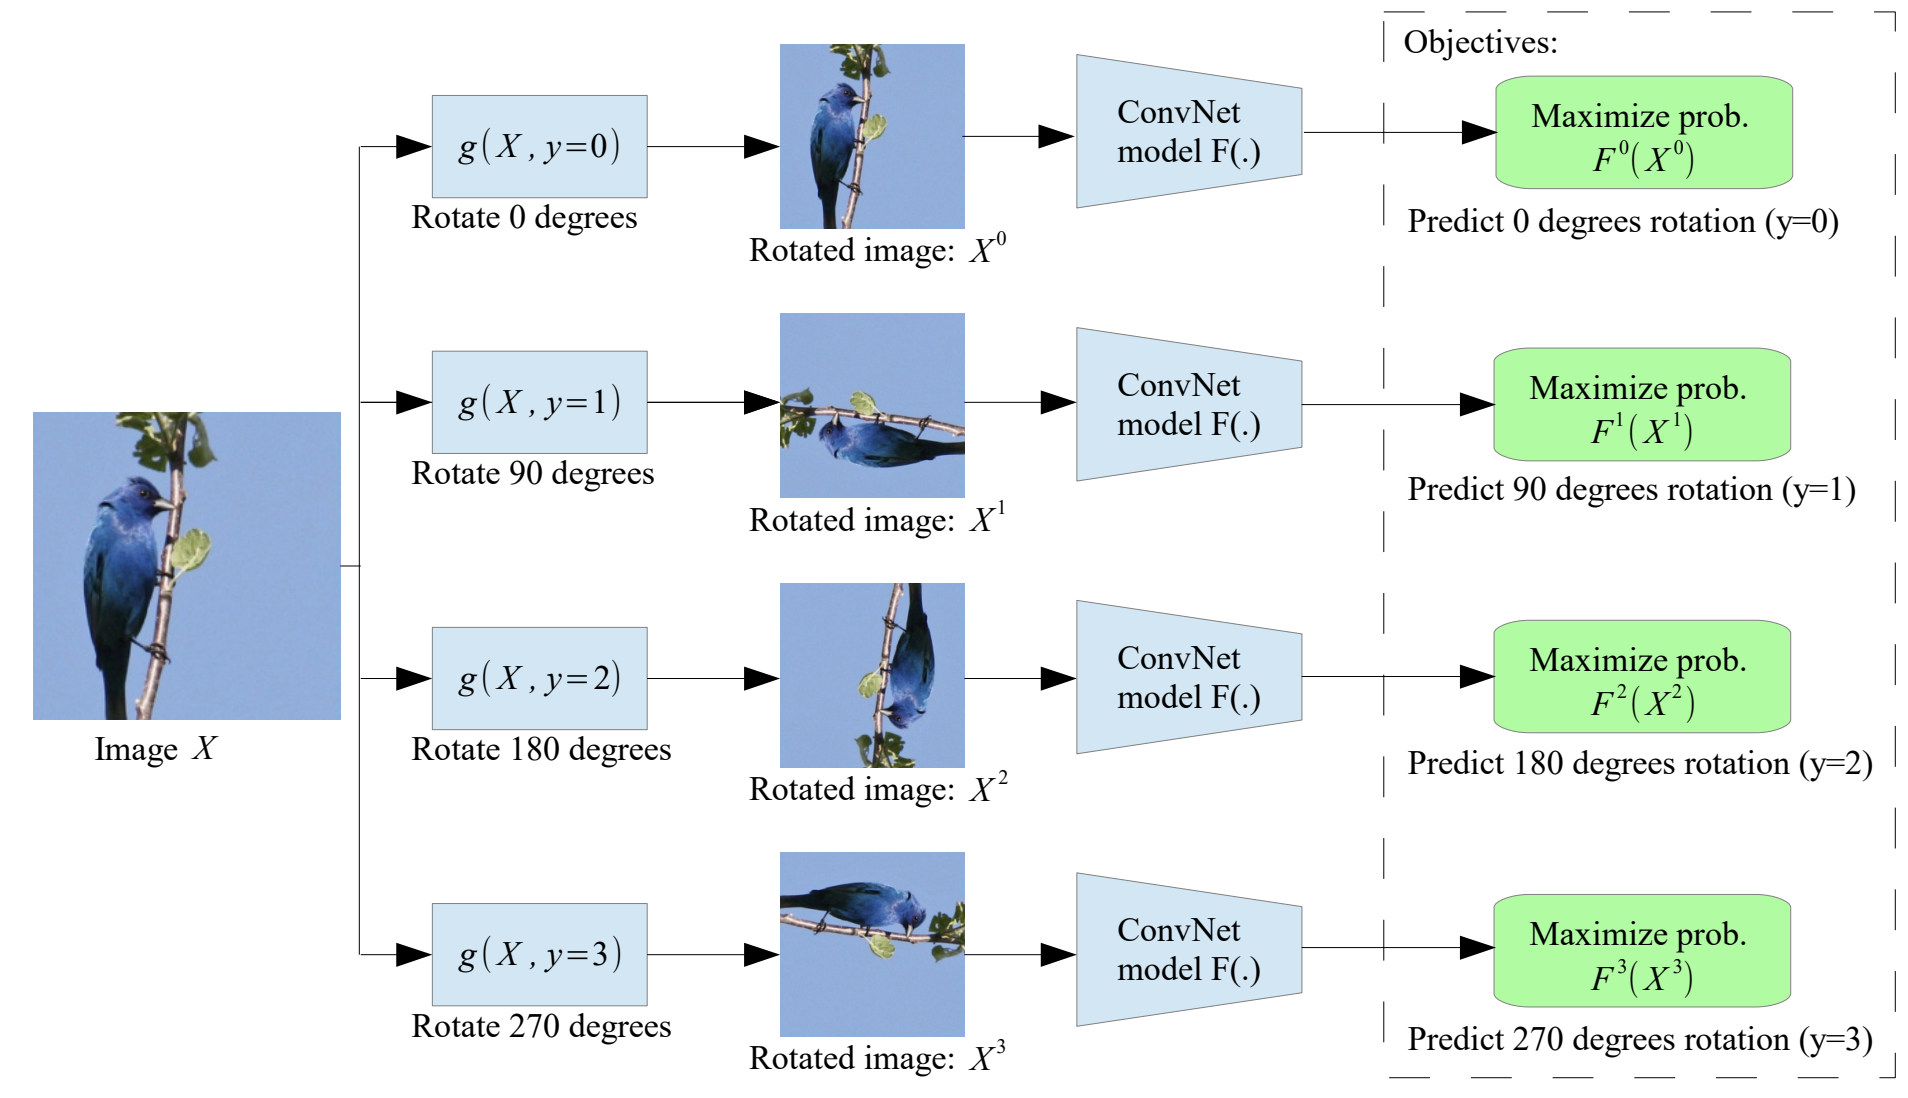
\includegraphics[width=1\linewidth,height=\textheight,keepaspectratio]{images/ssl/slide_33_1_img.png}
    \end{figure}

    \framebreak

    \begin{figure}
        \flushleft
        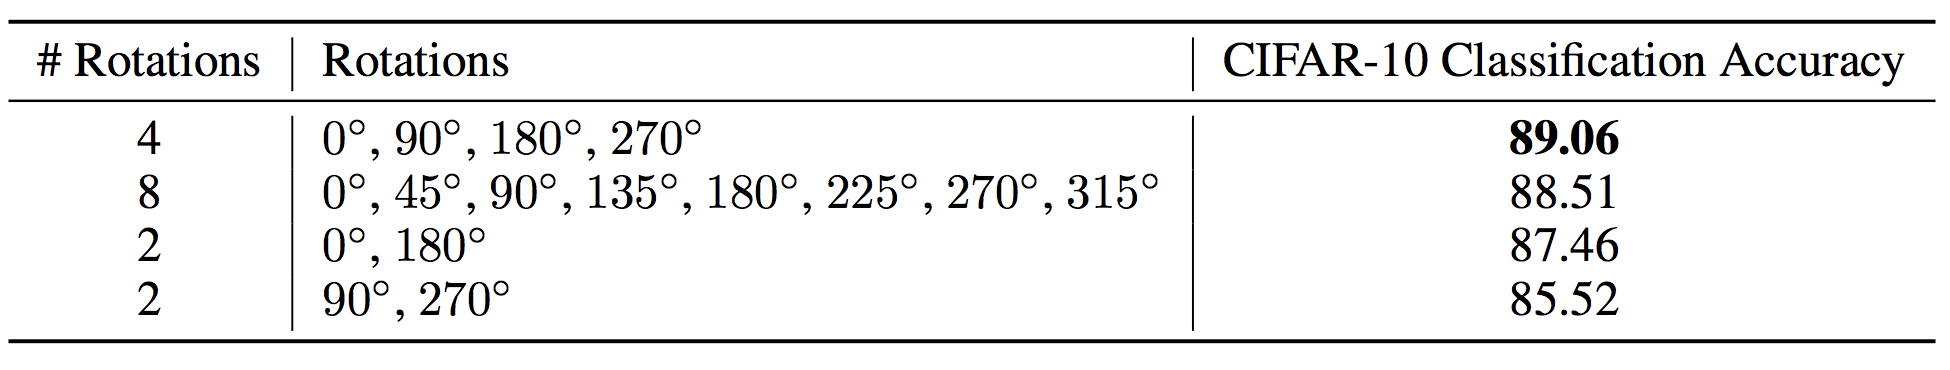
\includegraphics[width=1\linewidth,height=\textheight,keepaspectratio]{images/ssl/slide_34_1_img.png}
    \end{figure}

    \framebreak

    \textbf{Benefits:}
    \begin{itemize}
        \item Simple to implement and computationally inexpensive.
        \item Effective for learning global shape and semantic features.
        \item Can be used as a pretext task for downstream applications (e.g., image classification, object detection).
    \end{itemize}
    \textbf{References:}
    \begin{itemize}
        \item Gidaris, S., Singh, P., & Komodakis, N. (2018). Unsupervised Representation Learning by Predicting Image Rotations. \textit{ICLR 2018}.
    \end{itemize}
\end{frame}